\chapter{Project: A Programming Language}\label{language}

\epigraphhead[30]{
\epigraph{\hspace*{-.1cm}\itshape``The evaluator, which determines the meaning of expressions in a programming language, is just another program.''}%
{---Hal Abelson and Gerald Sussman, Structure and Interpretation of Computer Programs}
}\index{Abelson, Hal}\index{Sussman, Gerald}\index{SICP}\index{project chapter}

Building your own \index{programming language}programming language is surprisingly easy (as long as you do not aim too high) and very enlightening.

The main thing I want to show in this chapter is that there is no \index{magic}magic involved in building your own language. I've often felt that some human inventions were so immensely clever and complicated that I'd never be able to understand them. But with a little reading and experimenting, they often turn out to be quite mundane.\index{Egg language}\index{abstraction!in Egg}

We will build a programming language called Egg. It will be a tiny, simple language—but one that is powerful enough to express any computation you can think of. It will allow simple \index{abstraction}abstraction based on \index{function}functions.

\label{language.parsing}\section{Parsing}\index{parsing}\index{validation}\index{syntax!of Egg}

The most immediately visible part of a programming language is its \emph{syntax}, or notation. A \emph{parser} is a program that reads a piece of text and produces a data structure that reflects the structure of the program contained in that text. If the text does not form a valid program, the parser should point out the error.\index{special form}\index{function!application}

Our language will have a simple and uniform syntax. Everything in Egg is an \index{expression}expression. An expression can be the name of a binding, a number, a string, or an \emph{application}. Applications are used for function calls but also for constructs such as \lstinline`if` or \lstinline`while`.\index{double-quote character}\index{parsing}\index{escaping!in strings}\index{whitespace!syntax}

To keep the parser simple, strings in Egg do not support anything like backslash escapes. A string is simply a sequence of characters that are not double quotes, wrapped in double quotes. A number is a sequence of digits. Binding names can consist of any character that is not whitespace and that does not have a special meaning in the syntax.\index{comma character}\index{parentheses!arguments}

Applications are written the way they are in JavaScript, by putting parentheses after an expression and having any number of \index{argument}arguments between those parentheses, separated by commas.

\begin{lstlisting}
do(define(x, 10),
   if(>(x, 5),
      print("large"),
      print("small")))
\end{lstlisting}
\noindent\index{block}\index{syntax!of Egg}

The \index{uniformity}uniformity of the \index{Egg language}Egg language means that things that are \index{operator}operators in JavaScript (such as \lstinline`>`) are normal bindings in this language, applied just like other \index{function}functions. And since the syntax has no concept of a block, we need a \lstinline`do` construct to represent doing multiple things in sequence.\index{type property}\index{parsing}\index{data structure!tree}

The data structure that the parser will use to describe a program consists of \index{expression}expression objects, each of which has a \lstinline`type` property indicating the kind of expression it is and other properties to describe its content.\index{identifier}

Expressions of type \lstinline`"value"` represent literal strings or numbers. Their \lstinline`value` property contains the string or number value that they represent. Expressions of type \lstinline`"word"` are used for identifiers (names). Such objects have a \lstinline`name` property that holds the identifier's name as a string. Finally, \lstinline`"apply"` expressions represent applications. They have an \lstinline`operator` property that refers to the expression that is being applied, as well as an \lstinline`args` property that holds an array of argument expressions.

The \lstinline`>(x, 5)` part of the previous program would be represented like this:

\begin{lstlisting}
{
  type: "apply",
  operator: {type: "word", name: ">"},
  args: [
    {type: "word", name: "x"},
    {type: "value", value: 5}
  ]
}
\end{lstlisting}
\noindent\index{abstract syntax tree|see{syntax tree}}

Such a data structure is called a \emph{\index{syntax tree}syntax tree}. If you imagine the objects as dots and the links between them as lines between those dots, it has a \index{tree}treelike shape. The fact that expressions contain other expressions, which in turn might contain more expressions, is similar to the way tree branches split and split again.

\vskip 1.5ex
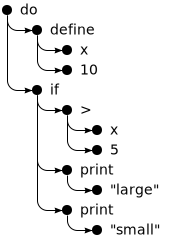
\includegraphics[width=5cm]{img/generated/syntax_tree.pdf}
\vskip 1.5ex\index{parsing}

Contrast this to the parser we wrote for the configuration file format in \hyperref[regexp.ini]{Chapter 9}, which had a simple structure: it split the input into lines and handled those lines one at a time. There were only a few simple forms that a line was allowed to have.\index{recursion}\index{nesting!of expressions}

Here we must find a different approach. Expressions are not separated into lines, and they have a recursive structure. Application expressions \emph{contain} other expressions.\index{elegance}

Fortunately, this problem can be solved very well by writing a parser function that is recursive in a way that reflects the recursive nature of the language.\index{parseExpression function}\index{syntax tree}

We define a function \lstinline`parseExpression`, which takes a string as input and returns an object containing the data structure for the expression at the start of the string, along with the part of the string left after parsing this expression. When parsing subexpressions (the argument to an application, for example), this function can be called again, yielding the argument expression as well as the text that remains. This text may in turn contain more arguments or may be the closing parenthesis that ends the list of arguments.

This is the first part of the parser:

\begin{lstlisting}
function parseExpression(program) {
  program = skipSpace(program);
  let match, expr;
  if (match = /^"([^"]*)"/.exec(program)) {
    expr = {type: "value", value: match[1]};
  } else if (match = /^\d+\b/.exec(program)) {
    expr = {type: "value", value: Number(match[0])};
  } else if (match = /^[^\s(),#"]+/.exec(program)) {
    expr = {type: "word", name: match[0]};
  } else {
    throw new SyntaxError("Unexpected syntax: " + program);
  }

  return parseApply(expr, program.slice(match[0].length));
}

function skipSpace(string) {
  let first = string.search(/\S/);
  if (first == -1) return "";
  return string.slice(first);
}
\end{lstlisting}
\noindent\index{skipSpace function}\index{whitespace!syntax}

Because Egg, like JavaScript, allows any amount of whitespace between its elements, we have to repeatedly cut the whitespace off the start of the program string. That is what the \lstinline`skipSpace` function helps with.\index{literal expression}\index{SyntaxError type}

After skipping any leading space, \lstinline`parseExpression` uses three \index{regular expression}regular expressions to spot the three atomic elements that Egg supports: strings, numbers, and words. The parser constructs a different kind of data structure depending on which one matches. If the input does not match one of these three forms, it is not a valid expression, and the parser throws an error. We use \lstinline`SyntaxError` instead of \lstinline`Error` as the exception constructor, which is another standard error type, because it is a little more specific—it is also the error type thrown when an attempt is made to run an invalid JavaScript program.\index{parseApply function}

We then cut off the part that was matched from the program string and pass that, along with the object for the expression, to \lstinline`parseApply`, which checks whether the expression is an application. If so, it parses a parenthesized list of arguments.

\begin{lstlisting}
function parseApply(expr, program) {
  program = skipSpace(program);
  if (program[0] != "(") {
    return {expr: expr, rest: program};
  }

  program = skipSpace(program.slice(1));
  expr = {type: "apply", operator: expr, args: []};
  while (program[0] != ")") {
    let arg = parseExpression(program);
    expr.args.push(arg.expr);
    program = skipSpace(arg.rest);
    if (program[0] == ",") {
      program = skipSpace(program.slice(1));
    } else if (program[0] != ")") {
      throw new SyntaxError("Expected ',' or ')'");
    }
  }
  return parseApply(expr, program.slice(1));
}
\end{lstlisting}
\noindent\index{parsing}

If the next character in the program is not an opening parenthesis, this is not an application, and \lstinline`parseApply` returns the expression it was given.\index{recursion}

Otherwise, it skips the opening parenthesis and creates the \index{syntax
tree}syntax
tree object for this application expression. It then recursively calls \lstinline`parseExpression` to parse each argument until a closing parenthesis is found. The recursion is indirect, through \lstinline`parseApply` and \lstinline`parseExpression` calling each other.

Because an application expression can itself be applied (such as in \lstinline`multiplier(2)(1)`), \lstinline`parseApply` must, after it has parsed an application, call itself again to check whether another pair of parentheses follows.\index{syntax tree}\index{Egg language}\index{parse function}

This is all we need to parse Egg. We wrap it in a convenient \lstinline`parse` function that verifies that it has reached the end of the input string after parsing the expression (an Egg program is a single expression), and that gives us the program's data structure.

\begin{lstlisting}
function parse(program) {
  let {expr, rest} = parseExpression(program);
  if (skipSpace(rest).length > 0) {
    throw new SyntaxError("Unexpected text after program");
  }
  return expr;
}

console.log(parse("+(a, 10)"));
// → {type: "apply",
//    operator: {type: "word", name: "+"},
//    args: [{type: "word", name: "a"},
//           {type: "value", value: 10}]}
\end{lstlisting}
\noindent\index{error message}

It works! It doesn't give us very helpful information when it fails and doesn't store the line and column on which each expression starts, which might be helpful when reporting errors later, but it's good enough for our purposes.

\section{The evaluator}\index{evaluate function}\index{evaluation}\index{interpretation}\index{syntax tree}\index{Egg language}

What can we do with the syntax tree for a program? Run it, of course! And that is what the evaluator does. You give it a syntax tree and a scope object that associates names with values, and it will evaluate the expression that the tree represents and return the value that this produces.

\begin{lstlisting}
const specialForms = Object.create(null);

function evaluate(expr, scope) {
  if (expr.type == "value") {
    return expr.value;
  } else if (expr.type == "word") {
    if (expr.name in scope) {
      return scope[expr.name];
    } else {
      throw new ReferenceError(
        `Undefined binding: ${expr.name}`);
    }
  } else if (expr.type == "apply") {
    let {operator, args} = expr;
    if (operator.type == "word" &&
        operator.name in specialForms) {
      return specialForms[operator.name](expr.args, scope);
    } else {
      let op = evaluate(operator, scope);
      if (typeof op == "function") {
        return op(...args.map(arg => evaluate(arg, scope)));
      } else {
        throw new TypeError("Applying a non-function.");
      }
    }
  }
}
\end{lstlisting}
\noindent\index{literal expression}\index{scope}

The evaluator has code for each of the \index{expression}expression types. A literal value expression produces its value. (For example, the expression \lstinline`100` just evaluates to the number 100.) For a binding, we must check whether it is actually defined in the scope and, if it is, fetch the binding's value.\index{function!application}

Applications are more involved. If they are a \index{special form}special form, like \lstinline`if`, we do not evaluate anything and pass the argument expressions, along with the scope, to the function that handles this form. If it is a normal call, we evaluate the operator, verify that it is a function, and call it with the evaluated arguments.

We use plain JavaScript function values to represent Egg's function values. We will come back to this \hyperref[language.egg_fun]{later}, when the special form called \lstinline`fun` is defined.\index{readability}\index{evaluate function}\index{recursion}\index{parsing}

The recursive structure of \lstinline`evaluate` resembles the similar structure of the parser, and both mirror the structure of the language itself. It would also be possible to integrate the parser with the evaluator and evaluate during parsing, but splitting them up this way makes the program clearer.\index{Egg language}\index{interpretation}

This is really all that is needed to interpret Egg. It is that simple. But without defining a few special forms and adding some useful values to the \index{environment}environment, you can't do much with this language yet.

\section{Special forms}\index{special form}\index{specialForms object}

The \lstinline`specialForms` object is used to define special syntax in Egg. It associates words with functions that evaluate such forms. It is currently empty. Let's add \lstinline`if`.

\begin{lstlisting}
specialForms.if = (args, scope) => {
  if (args.length != 3) {
    throw new SyntaxError("Wrong number of args to if");
  } else if (evaluate(args[0], scope) !== false) {
    return evaluate(args[1], scope);
  } else {
    return evaluate(args[2], scope);
  }
};
\end{lstlisting}
\noindent\index{conditional execution}\index{ternary operator}\index{?: operator}\index{conditional operator}

Egg's \lstinline`if` construct expects exactly three arguments. It will evaluate the first, and if the result isn't the value \lstinline`false`, it will evaluate the second. Otherwise, the third gets evaluated. This \lstinline`if` form is more similar to JavaScript's ternary \lstinline`?:` operator than to JavaScript's \lstinline`if`. It is an expression, not a statement, and it produces a value, namely, the result of the second or third argument.\index{Boolean}

Egg also differs from JavaScript in how it handles the condition value to \lstinline`if`. It will not treat things like zero or the empty string as false, only the precise value \lstinline`false`.\index{short-circuit evaluation}

The reason we need to represent \lstinline`if` as a special form, rather than a regular function, is that all arguments to functions are evaluated before the function is called, whereas \lstinline`if` should evaluate only \emph{either} its second or its third argument, depending on the value of the first.

The \lstinline`while` form is similar.

\begin{lstlisting}
specialForms.while = (args, scope) => {
  if (args.length != 2) {
    throw new SyntaxError("Wrong number of args to while");
  }
  while (evaluate(args[0], scope) !== false) {
    evaluate(args[1], scope);
  }

  // Since undefined does not exist in Egg, we return false,
  // for lack of a meaningful result.
  return false;
};
\end{lstlisting}
\noindent

Another basic building block is \lstinline`do`, which executes all its arguments from top to bottom. Its value is the value produced by the last argument.

\begin{lstlisting}
specialForms.do = (args, scope) => {
  let value = false;
  for (let arg of args) {
    value = evaluate(arg, scope);
  }
  return value;
};
\end{lstlisting}
\noindent\index{= operator!in Egg}\index{binding!in Egg}

To be able to create bindings and give them new values, we also create a form called \lstinline`define`. It expects a word as its first argument and an expression producing the value to assign to that word as its second argument. Since \lstinline`define`, like everything, is an expression, it must return a value. We'll make it return the value that was assigned (just like JavaScript's \lstinline`=` operator).

\begin{lstlisting}
specialForms.define = (args, scope) => {
  if (args.length != 2 || args[0].type != "word") {
    throw new SyntaxError("Incorrect use of define");
  }
  let value = evaluate(args[1], scope);
  scope[args[0].name] = value;
  return value;
};
\end{lstlisting}
\noindent

\section{The environment}\index{Egg language}\index{evaluate function}\index{binding!in Egg}

The \index{scope}scope accepted by \lstinline`evaluate` is an object with properties whose names correspond to binding names and whose values correspond to the values those bindings are bound to. Let's define an object to represent the \index{global scope}global scope.

To be able to use the \lstinline`if` construct we just defined, we must have access to \index{Boolean}Boolean values. Since there are only two Boolean values, we do not need special syntax for them. We simply bind two names to the values \lstinline`true` and \lstinline`false` and use them.

\begin{lstlisting}
const topScope = Object.create(null);

topScope.true = true;
topScope.false = false;
\end{lstlisting}
\noindent

We can now evaluate a simple expression that negates a Boolean value.

\begin{lstlisting}
let prog = parse(`if(true, false, true)`);
console.log(evaluate(prog, topScope));
// → false
\end{lstlisting}
\noindent\index{arithmetic}\index{Function constructor}

To supply basic \index{arithmetic}arithmetic and \index{comparison}comparison \index{operator}operators, we will also add some function values to the \index{scope}scope. In the interest of keeping the code short, we'll use \lstinline`Function` to synthesize a bunch of operator functions in a loop, instead of defining them individually.

\begin{lstlisting}
for (let op of ["+", "-", "*", "/", "==", "<", ">"]) {
  topScope[op] = Function("a, b", `return a ${op} b;`);
}
\end{lstlisting}
\noindent

A way to \index{output}output values is also useful, so we'll wrap \lstinline`console.log` in a function and call it \lstinline`print`.

\begin{lstlisting}
topScope.print = value => {
  console.log(value);
  return value;
};
\end{lstlisting}
\noindent\index{parsing}\index{run function}

That gives us enough elementary tools to write simple programs. The following function provides a convenient way to parse a program and run it in a fresh scope:

\begin{lstlisting}
function run(program) {
  return evaluate(parse(program), Object.create(topScope));
}
\end{lstlisting}
\noindent\index{Object.create function}\index{prototype}

We'll use object prototype chains to represent nested scopes so that the program can add bindings to its local scope without changing the top-level scope.

\begin{lstlisting}
run(`
do(define(total, 0),
   define(count, 1),
   while(<(count, 11),
         do(define(total, +(total, count)),
            define(count, +(count, 1)))),
   print(total))
`);
// → 55
\end{lstlisting}
\noindent\index{summing example}\index{Egg language}

This is the program we've seen several times before, which computes the sum of the numbers 1 to 10, expressed in Egg. It is clearly uglier than the equivalent JavaScript program—but not bad for a language implemented in less than 150 \index{lines of code}lines of code.

\label{language.egg_fun}\section{Functions}\index{function}\index{Egg language}

A programming language without functions is a poor programming language indeed.

Fortunately, it isn't hard to add a \lstinline`fun` construct, which treats its last argument as the function's body and uses all arguments before that as the names of the function's parameters.

\begin{lstlisting}
specialForms.fun = (args, scope) => {
  if (!args.length) {
    throw new SyntaxError("Functions need a body");
  }
  let body = args[args.length - 1];
  let params = args.slice(0, args.length - 1).map(expr => {
    if (expr.type != "word") {
      throw new SyntaxError("Parameter names must be words");
    }
    return expr.name;
  });

  return function() {
    if (arguments.length != params.length) {
      throw new TypeError("Wrong number of arguments");
    }
    let localScope = Object.create(scope);
    for (let i = 0; i < arguments.length; i++) {
      localScope[params[i]] = arguments[i];
    }
    return evaluate(body, localScope);
  };
};
\end{lstlisting}
\noindent\index{local scope}

Functions in Egg get their own local scope. The function produced by the \lstinline`fun` form creates this local scope and adds the argument bindings to it. It then evaluates the function body in this scope and returns the result.

\begin{lstlisting}
run(`
do(define(plusOne, fun(a, +(a, 1))),
   print(plusOne(10)))
`);
// → 11

run(`
do(define(pow, fun(base, exp,
     if(==(exp, 0),
        1,
        *(base, pow(base, -(exp, 1)))))),
   print(pow(2, 10)))
`);
// → 1024
\end{lstlisting}
\noindent

\section{Compilation}\index{interpretation}\index{compilation}

What we have built is an interpreter. During evaluation, it acts directly on the representation of the program produced by the parser.\index{efficiency}\index{performance}\index{binding!definition}\index{memory!speed}

\emph{Compilation} is the process of adding another step between the parsing and the running of a program, which transforms the program into something that can be evaluated more efficiently by doing as much work as possible in advance. For example, in well-designed languages it is obvious, for each use of a binding, which binding is being referred to, without actually running the program. This can be used to avoid looking up the binding by name every time it is accessed, instead directly fetching it from some predetermined memory location.

Traditionally, \index{compilation}compilation involves converting the program to \index{machine code}machine code, the raw format that a computer's processor can execute. But any process that converts a program to a different representation can be thought of as compilation.\index{simplicity}\index{Function constructor}\index{transpilation}

It would be possible to write an alternative \index{evaluation}evaluation strategy for Egg, one that first converts the program to a JavaScript program, uses \lstinline`Function` to invoke the JavaScript compiler on it, and then runs the result. When done right, this would make Egg run very fast while still being quite simple to implement.

If you are interested in this topic and willing to spend some time on it, I encourage you to try to implement such a compiler as an exercise.

\section{Cheating}\index{Egg language}

When we defined \lstinline`if` and \lstinline`while`, you probably noticed that they were more or less trivial wrappers around JavaScript's own \lstinline`if` and \lstinline`while`. Similarly, the values in Egg are just regular old JavaScript values.

If you compare the implementation of Egg, built on top of JavaScript, with the amount of work and complexity required to build a programming language directly on the raw functionality provided by a machine, the difference is huge. Regardless, this example ideally gave you an impression of the way \index{programming language}programming languages work.

And when it comes to getting something done, cheating is more effective than doing everything yourself. Though the toy language in this chapter doesn't do anything that couldn't be done better in JavaScript, there \emph{are} situations where writing small languages helps get real work done.

Such a language does not have to resemble a typical programming language. If JavaScript didn't come equipped with regular expressions, for example, you could write your own parser and evaluator for regular expressions.\index{artificial intelligence}

Or imagine you are building a giant robotic \index{dinosaur}dinosaur and need to program its \index{behavior}behavior. JavaScript might not be the most effective way to do this. You might instead opt for a language that looks like this:

\begin{lstlisting}
behavior walk
  perform when
    destination ahead
  actions
    move left-foot
    move right-foot

behavior attack
  perform when
    Godzilla in-view
  actions
    fire laser-eyes
    launch arm-rockets
\end{lstlisting}
\noindent\index{expressivity}

This is what is usually called a \emph{\index{domain-specific language}domain-specific language}, a language tailored to express a narrow domain of knowledge. Such a language can be more expressive than a general-purpose language because it is designed to describe exactly the things that need to be described in its domain, and nothing else.

\section{Exercises}

\subsection{Arrays}\index{Egg language}\index{arrays in egg (exercise)}\index{array!in Egg}

Add support for arrays to Egg by adding the following three functions to the top scope: \lstinline`array(...values)` to construct an array containing the argument values, \lstinline`length(array)` to get an array's length, and \lstinline`element(array, n)` to fetch the n\textsuperscript{th} element from an array.

\subsection{Closure}\index{closure}\index{function!scope}\index{closure in egg (exercise)}

The way we have defined \lstinline`fun` allows functions in Egg to reference the surrounding scope, allowing the function's body to use local values that were visible at the time the function was defined, just like JavaScript functions do.

The following program illustrates this: function \lstinline`f` returns a function that adds its argument to \lstinline`f`'s argument, meaning that it needs access to the local \index{scope}scope inside \lstinline`f` to be able to use binding \lstinline`a`.

\begin{lstlisting}
run(`
do(define(f, fun(a, fun(b, +(a, b)))),
   print(f(4)(5)))
`);
// → 9
\end{lstlisting}
\noindent

Go back to the definition of the \lstinline`fun` form and explain which mechanism causes this to work.

\subsection{Comments}\index{hash character}\index{Egg language}\index{comments in egg (exercise)}

It would be nice if we could write \index{comment}comments in Egg. For example, whenever we find a hash sign (\lstinline`#`), we could treat the rest of the line as a comment and ignore it, similar to \lstinline`//` in JavaScript.\index{skipSpace function}

We do not have to make any big changes to the parser to support this. We can simply change \lstinline`skipSpace` to skip comments as if they are \index{whitespace}whitespace so that all the points where \lstinline`skipSpace` is called will now also skip comments. Make this change.

\subsection{Fixing scope}\index{binding!definition}\index{assignment}\index{fixing scope (exercise)}

Currently, the only way to assign a binding a value is \lstinline`define`. This construct acts as a way both to define new bindings and to give existing ones a new value.\index{local binding}

This \index{ambiguity}ambiguity causes a problem. When you try to give a nonlocal binding a new value, you will end up defining a local one with the same name instead. Some languages work like this by design, but I've always found it an awkward way to handle \index{scope}scope.\index{ReferenceError type}

Add a special form \lstinline`set`, similar to \lstinline`define`, which gives a binding a new value, updating the binding in an outer scope if it doesn't already exist in the inner scope. If the binding is not defined at all, throw a \lstinline`ReferenceError` (another standard error type).\index{hasOwnProperty method}\index{prototype}\index{getPrototypeOf function}

The technique of representing scopes as simple objects, which has made things convenient so far, will get in your way a little at this point. You might want to use the \lstinline`Object.getPrototypeOf` function, which returns the prototype of an object. Also remember that scopes do not derive from \lstinline`Object.prototype`, so if you want to call \lstinline`hasOwnProperty` on them, you have to use this clumsy expression:

\begin{lstlisting}
Object.prototype.hasOwnProperty.call(scope, name);
\end{lstlisting}
\noindent
